\documentclass[12pt,letterpaper]{article}
\usepackage{anysize}
\usepackage{amsmath}
\marginsize{2cm}{2cm}{1cm}{1cm}
\usepackage{listings}
\usepackage{cite}
\usepackage{caption}
\usepackage{upquote}
\usepackage{xcolor}
\usepackage{xcolor}

\usepackage{graphicx}


\begin{document}

\begin{titlepage}
    \vspace*{4cm}
    \begin{flushleft}
    {\huge
        CS519 Project 2\\[.5cm]
    }
    {\large
        Elliptical Dots
    }
    \end{flushleft}
    \vfill
    \rule{5in}{.5mm}\\
    Li Li

\end{titlepage}
\section{source files}
There are only two files labone.rib and labone.sl.
\section{a simple explanation}
What I did are:
\begin{itemize}
\item Follow the hint in \bf {Stripes, Rings and Dots}. Create an
  eclipse formula. For given parameter of the formula, I replaced Diam
  with Ad and Bd to represent the eclipse. Other stuff just remain the same.
\item Load a vase.rib to represent my object. That is just replace the
  sphere in rib file with those tons of polygons.
\item After these two steps it came out with very tiny dots on the
  objects, even i chance my Ad and Bd. The dots can not grow bigger,
  actually stay in as large as in a single face. Then I went to the
  notes and find out it may be deal with u,v. After I changed my \bf {up} to
  2*xcomp(P), which is X component of a point. And similarly done
  changes on \bf {vp}. After that it gives out the desired image.
\end{itemize}
\section{result}
\begin{center}
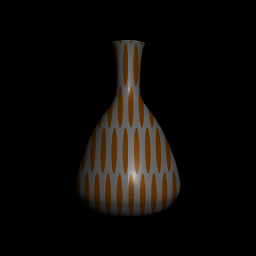
\includegraphics[scale = 1.5]{labone.png}
\end{center}


\end {document}
